\section{View Maintenance System} 
\label{sec:view_maintenance_system} 

In this section, we build and integrate the VMS with KV-store -- always 
keeping consistency requirements in mind. The
section is organized as follows: we discuss the design of the 
VMS and its components. We depict the processing of an operation through 
the VMS architecture. We analyse consistency of VMS in a dynamic context. 
Finally, we discuss fault tolerance mechanisms and the supported view
types in VMS. 




%A \textit{view expression} defines the operations that are to be
%applied to one or more base tables to materialize a \textit{view} over
%the base data (e.g., selection, aggregation or join).  We refer to the
%materialized view as the \textit{view table} as it simply is a table
%in the KV-store, persisted like any another base table and potentially
%split across a number of nodes. Base tables and derived view tables
%can be hosted alone or together on the same or different nodes.  As
%clients perform updates against base tables, derived view tables
%become stale. It is the job of the \textit{view maintenance system}
%(VMS) to update view tables as base tables change. VMS is represented
%by the black blocks in the figure. It receives base table operations
%and applies them in order to view tables. VMS decouples base table
%management from view table materialization. If desired, view tables
%could be stored at a completely different set of nodes or at another
%system instance altogether. We now describe all components that make
%up VMS.

\subsection{Design}

Figure~\ref{fig:view_maintenance_system} provides a system overview. The 
VMS consists of a \textit{coordinator} and an arbitrary number of 
\textit{subsystems} (Sub). The coordinator controls load balancing and 
recovery mechanisms, whereas the subsystems -- more specifically the 
\textit{view managers} (VMs) in the subsystems -- update the view tables. The input 
of the VMS is a set of operation streams ($ts_1$,$ts_2$..$ts_n$); 
each resulting from a KV-store node (cf. Figure~\ref{fig:kv_model}). 
Thereby, one subsystem of VMS manages one stream of operations exclusively.  
The subsystem distributes incoming operations to the view managers. The 
number of view managers in a subsystem is scalable. New view 
managers can be \textit{assigned} to or \textit{removed} from the 
subsystem. The coordinator can also re-assign view managers from one 
subsystem to another. 

 The \textbf{view manager} is light-weight and deployed in large 
numbers to accommodate the view update load. It applies base table 
operations to view tables. A view manager can only belong to a 
single subsystem. The subsystem feeds the view manager with operations; the
view manager processes the operations in order.  A view manager is the unit of 
scalability for VMS. We keep VMs stateless -- they should be exchangeable 
at any time -- To minimize dependency. Given a number of view definitions 
and a sequence of operations, the view manager is always able to execute 
any view table update at any host. 


\begin{figure}
  \centering
    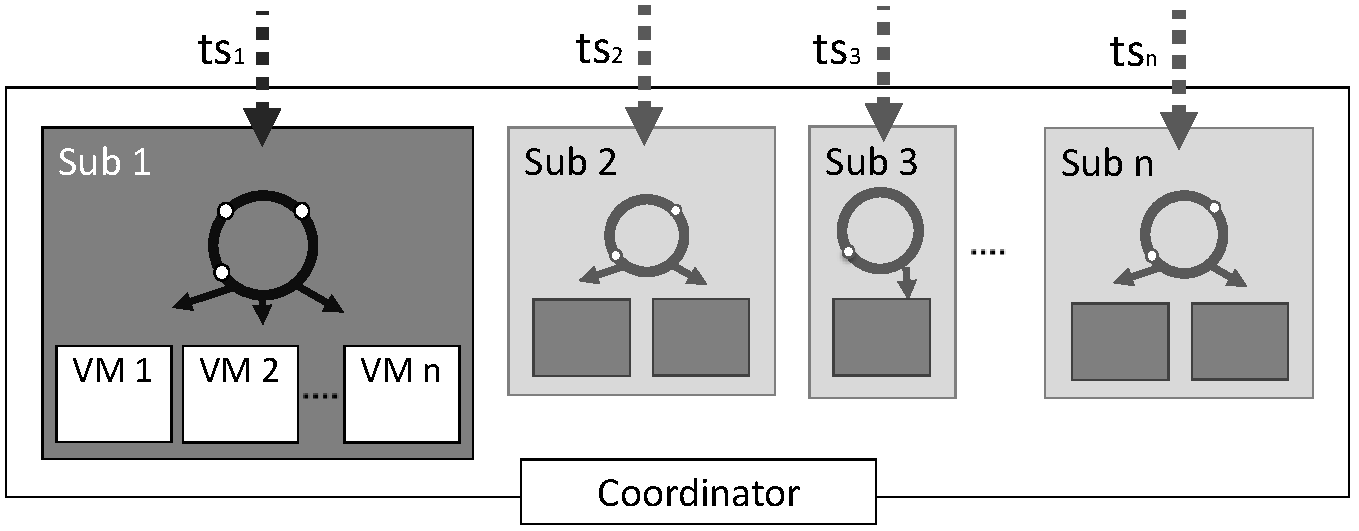
\includegraphics[width=\linewidth]{figures/ViewMaintenanceSystem}
    \caption{View Maintenance System}
    \label{fig:view_maintenance_system}
\end{figure}

Our design bares the following benefits: (i) 
Hundreds of views may be updated in consequence of one base table 
operation. As VMS exceeds its performance limits, additional VMs can be 
assigned (below, we show this experimentally). (ii) VMs introduce 
flexibility to the system architecture: VMs of a subsystem can be hosted 
together on the same node; or each of them can be hosted at a different 
node. (iii) Also, VMs can be reassigned from one subsystem to another in 
times of changing base table update load. (iv) If a VM crashes, another 
VM can take over and continue processing the operation stream. 



The \textit{coordinator} manages the component configuration of VMS. It 
sends commands to the remaining components and induces certain actions. 
For example, if a VM has to be assigned to a node, the coordinator sends 
an assignment command. Likewise, the coordinator reacts to system events 
and takes care of the system state. It monitors the VMS state by relying 
on the distributed configuration service \textit{Zookeeper}. Every VM 
instance is represented in Zookeeper by an \textit{ephemeral node}. In 
case of a VM crash, the ephemeral node is destroyed and the coordinator 
receives an event. It then performs different recovery steps to 
guarantee error recovery. 


\subsection{Operation processing} 
\label{subsec:update_processing} 

%This section details the inner workings of VMS.  We begin by detailing
%the life of a client request as it passes from the a client to the
%base table via the KV-store and to the view table via VMS. 

When receiving operations from the stream, the subsystem distributes 
them to the set of assigned view managers. Thereby, it applies 
the principles of \textit{consistent hashing} to route the operations. 
Routing the operations allows for maximal concurrency, while simultaneously
guaranteeing timeline consistency (cf. Section~\ref{subsubsec:record_timeline}).  
The subsystem will distribute operations uniformly -- but it will send 
multiple operations on the same row key always to the same view manager. 


Consistent hashing is realized as follows: the 
subsystem maintains a hash-ring (cf. Figure~\ref{fig:review_consistency}) 
where it places a node for every 
assigned view manager (it applies a hash-function to the view managers 
name to determine the place). As the base table operations stream in, the 
subsystem extracts their row keys. Now, the subsystem applies 
the hash-function to the row key and determines the place on the 
hash-ring. Starting at this point, the subsystem travels clockwise until 
it hits the first node of a view manager -- meaning this view manager is 
responsible for processing. The subsystem sends the operation to this view 
manager and continues its work. 

Similar to the KV-store, the view manager runs its own transaction log,
called \textit{VM log}.  Before processing the operations, the view manager
writes them to the VM log, located at the file system. Here the VM log is 
replicated and can be used for recovery as soon as the view manager crashes.

To access and update the view table, the view manager acts as a client 
to the KV-store, using the standard KV-API. Given a client operation, the 
VM retrieves the view definitions of the views defined over the updated 
base table, runs the update programs, and 
submits view table updates via the KV-API. All view table definitions 
are stored in a meta-table in the KV-store keyed on base table name. 
View table definitions are cached by a VM. Once the VM knows the 
affected view tables and their definitions, it runs the view update 
logic and submits view table changes via the KV-API. Depending on the 
view type maintained, the VM has to query the view table as part of the 
update logic, which we detail below. 

To full fill the atomic update requirement (cf. 
Section~\ref{subsubsec:atomic_update}), we use a test-and-set 
mechanism.~\footnote{In HBase a \texttt{checkAndPut} method is provided 
to realize this mechanism. Most KV-stores offer a similar abstraction.} 
When updating a table record, a caller sees (tests) whether a record has 
been concurrently modified between a read and an update. Revisiting 
Example~2, let $VM_2$ retrieve value $(x1, \{(col_1, a)\})$. Then, it 
computes $(x1,\{(col_1,a+c)\})$ trying to put the new value, while 
testing for the old value $a$. The test-and-set fails because the old 
record value changed concurrently to $a+b$. Thus, $VM_2$ fetches the 
updated value again and re-computes $(x1,\{(col_1,a+b+c)\})$. This time 
the test-and-set succeeds and the record is written. 

After a view table has been updated, the VM persists the current state of
work -- that is, the \textit{sequence number} of the last processed client 
operation and the name of the updated view table. The state is stored into 
a field in Zookeeper, such that the coordinator can restore the information
 in case of a crash. Then, a new view manager can 
resume the work from this point. 




\begin{figure}
  \centering
    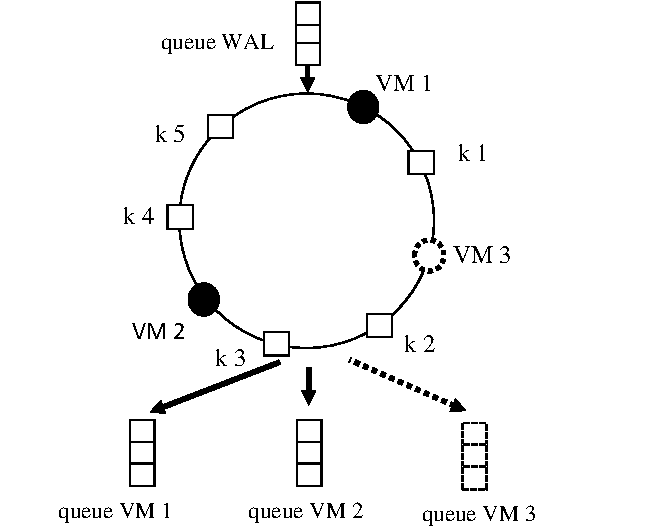
\includegraphics[width=\linewidth]{figures/ReviewConsistency}
    \caption{Subsystem set-up}
    \label{fig:review_consistency}
\end{figure}



\subsection{Dynamic Consistency} 


By now, consistency is guaranteed through the design of VMS. Consistent 
hashing ensures the record timeline during maintenance. But the VMS achieves
these guarantees only in a static set-up -- a fixed number of nodes and view 
managers is assumed. Switching to a dynamic context (and allowing the VMS to 
assign and withdraw view managers; or allowing the KV-store to add and 
remove nodes, move key-ranges, etc.) makes securing consistency difficult 
again. The following example shows why:


\textit{Example 3:} Consider a subsystem set-up as shown in 
Figure~\ref{fig:review_consistency}. Two view managers $VM_1$ and $VM_2$ 
are already assigned to the subsystem: they are responsible for a 
certain range on the hash-ring; queues are feeding them with 
incoming client operations. Assume a client performing a put operation $t_1(A(k_1, 
\{..\}))$ to a base table that is managed by the view managers. Further 
assume the subsystem selects $VM_2$ as the next responsible view manager 
for $t_1$. Then, $t_1$ is put to the queue of $VM_2$. Now assume, a view 
manager $VM_3$ is assigned to the subsystem and that $VM_3$ acquires the 
responsibility for key $k_1$. It is inserted into the hash-ring and a 
new queue is created. In a next step, a client sends an operation $t_2 
(A(k_1, \{..\}))$ to the same key. Because responsibility has changed, 
the operation is now added to the queue of $VM_3$. Considering, that 
$VM_3$ has just been added, it's queue is comparatively empty and hence 
processing very fast. It is likely to happen that $VM_3$ processes $t_2$ 
before $VM_2$ can process $t_1$. Because both operations refer to the 
same base record, the timeline of the record is broken. As explained 
before, this has to be prevented in order to preserve convergence of 
views. 

Thus, we now refine the behaviour of VMS in a dynamic context. First, we discuss the 
dynamics related to VMS actions (Table~\ref{tab:vms_events}); second, we discuss 
the dynamics related to KV-store events (Table~\ref{tab:kvs_a_events}).




\subsubsection{Dynamics VMS} 

 In Table~\ref{tab:vms_events} all VMS actions are shown. Some of them 
are not relevant to the consistency discussion. Adding a view manager to 
VMS (or removing it from VMS) does not affect the view maintenance 
process. The reassign action is a logical combination of a withdraw 
(from the old subsystem) and an assign (to the new subsystem). Thus, we 
now refine the assign and withdraw action of VMS. 




\begin{table}
\rowcolors{2}{gray!10}{gray!30}
\setlength{\belowrulesep}{0pt}
\setlength{\aboverulesep}{0pt}
\setlength\extrarowheight{2pt}
\begin{center}
\begin{tabular}{l l l}
\toprule
Component & action & method \\
\midrule
View Manager & add & \textit{addViewManager()}  \\
 & remove & \textit{removeViewManager()}    \\
 & assign & \textit{assignViewManager()}  \\
 & withdraw & \textit{withdrawViewManager()}    \\
  & re-assign & \textit{reassignViewManager()}    \\
\bottomrule 
\end{tabular}
\caption{VMS actions}
\label{tab:vms_events}
\end{center}
\end{table}


The solution we suggest, is using so called \textit{markers}. Markers 
identify whether a view manager has completed the processing of all 
operations (that were sent before) and, thus, allow the secure assignment 
and removal of view managers. Markers are sent just like client 
operations to the view manager: they are inserted into the queue of the 
view manager and become a part of the operation stream. When the 
view manager reads an operation and recognizes a marker, it replies with 
an acknowledgement back to the subsystem. 

To realize the marker 
mechanism, we adapted parts of the subsystem and VM implementation. 
The logic on the subsystem side is slightly more subtle and in the following 
we base our description on a set of primitive operations. These include 
methods that are needed by the subsystem to assign (or withdraw) VMs to (or 
from) itself: (i) $createQueue(vm)$ creates a new queue for a particular view 
manager and (ii) $deleteQueue(vm)$ removes an existing queue for a particular 
view manager at the subsystem. The queue for a VM can only be deleted, if it is empty and no 
operation is queued. (iii) $queue(vm, operation/marker)$ inserts, either a 
base table operation, or a marker into the queue of a particular view manager. 
The methods (iv) $activateQueue(vm)$ and (v) $deactivateQueue(vm)$ start or 
stop the sending thread that keeps transferring the operations in the queue 
for a particular VM. A view manager can be added to the hash ring by (vi) 
$insertHash(vm)$, or removed from the hash ring by (vii) $removeHash(vm)$. 



\noindent
\textit{Assign view manager -- } When a view manager is assigned, it 
is added to the hash-ring of the subsystem. Unless the hash-ring 
is empty, the new view manager is assigned a key region that is, at the same 
time, withdrawn from another view manager. In 
Figure~\ref{fig:review_consistency}, a view maintenance process of a subsystem 
is shown. Recall, that the subsystem selects the responsible view manager by 
applying the consistent hash function. The operation is then inserted 
into the corresponding queue. 


We change the assignment procedure by adding the marker-based acknowledgement 
mechanism (cf. Algorithm~\ref{alg:assignvm}). The algorithm is executed 
synchronously and if another assignment procedure is called on the subsystem, 
it has to wait, until the first operation has terminated.
%
%\renewcommand\alglinenumber[1]%
% {\ifodd\value{ALG@line}\relax
%  \noindent{\color{yellow}\leaders\vrule\hskip\linewidth\hbox{}\hskip-\linewidth\hbox{}}%
%  \fi
%\footnotesize\arabic{ALG@line}}

  
\begin{algorithm}
\caption{Secure assignment procedure at subsystem}
\label{alg:assignvm}
\begin{algorithmic}[5]
\Procedure{$assignVm$}{$vm_a, VM_{sub}$}
\State $createQueue(vm_a)$\Comment{create queue}
\State $insertHash(vm_a)$\Comment{add VM to hashring}
\ForAll{$vm \in VM_{sub}$}
\State $queue(vm, m_a)$\Comment{queue markers}	
\EndFor
\ForAll{$vm \in VM_{sub}$}\Comment{wait for acks}	
\State $receiveMessage(vm)$	
\EndFor
\State $activateQueue(vm_a)$\Comment{activate queue}	
\EndProcedure
\end{algorithmic}
\end{algorithm}
  
The procedure $assignVm$ takes two parameters: $vm_a$, the view manager 
that should be assigned to the subsystem, and $VM_{sub}$, a set of view 
managers that are already assigned to the subsystem. The algorithm 
creates a queue for $vm_a$ and inserts it into the hash-ring. Then, it 
queues a marker $m_a$ to all assigned VMs ($VM_{sub}$). After the 
subsystem has received acknowledgements from all VMs, it is guaranteed 
that no operation in the key range of the newly added view manager 
$vm_a$ is still pending. Referring back to Example~3: The timeline of 
$k_1$ can not be changed any more. Operation $t_2$ has to wait in the 
queue of $VM_3$, until $VM_2$ acknowledges the processing of $t_1$ 
because the queue of $VM_3$ is activated only after the marker has been 
acknowledged and this, in turn, implies that operation $t_1$ has been 
processed. 


\noindent
\textit{Withdraw view manager -- }During a withdraw procedure, 
consistency can be violated, likewise. At the moment where a view manager is 
withdrawn, i.e. removed from the hash-ring, its queue might still contain 
operations. If another view manager that acquires the key range is fast 
enough, it might processes operations before the withdrawn view manager 
has finished. Again, the timeline of base records is changed. In order 
to prevent inconsistency, we design Algorithm~\ref{alg:withdrawvm} 
analogous to Algorithm \ref{alg:assignvm}. It takes two parameters: 
$vm_w$, the view manager that should be withdrawn from the subsystem, 
and $VM_{sub}$, the set of view managers that is assigned to the subsystem. 


\begin{algorithm}
\caption{Secure withdraw procedure at subsystem}
\label{alg:withdrawvm}
\begin{algorithmic}[5]
\Procedure{$withdrawVm$}{$vm_w, VM_{sub}$}
\ForAll{$vm \in VM_{sub} \wedge vm \neq vm_w$}	
\State $deactivateQueue(vm)$\Comment{deactivate queues}
\EndFor
\State $removeHash(vm_w)$\Comment{redirect operations}
\State $queueMarker(vm_w, m_w)$
\ForAll{$vm \in VM_{sub}$}
\State $receiveMessage(vm)$\Comment{wait for acks}		
\EndFor
\State $removeQueue(vm_w)$
\ForAll{$vm \in VM$}\Comment{activate queues again}	
\State $activateQueue(vm)$
\EndFor
\EndProcedure
\end{algorithmic}
\end{algorithm}

First, the queues of the view managers that possibly increase their 
key range on the hash-ring (i.e., all other VMs) are deactivated. Then, 
a marker $m_w$ is queued to the view manager that is withdrawn. If the 
view manager has acknowledged the marker, the region server knows, that 
all operations have been processed. It removes the queue of the view 
manager and re-activates the queues of all view managers. 

\subsubsection{Dynamics KV-Store}
\label{subsubsec:dynamics_kv_store} 

 In Table~\ref{tab:vms_events} all KV-store events are depicted. Again we
 can exclude some of them from the consistency discussion. Adding a node to
 KV-store is not critical. The VMS just creates a subsystem for the new
 node and assigns view managers to it -- which start processing the client 
 operations of the new node. Removing a node from KV-store is also not 
 critical, as the key ranges on that node are either closed or moved to
 another node. The VMS continues reading client operations until the end 
 of the node's transaction log (as the file is still available) and then, 
 securely reassigns the view managers to another subsystem. 

\textit{Moving regions -- } Once in a while, the KV-store moves key 
ranges from one node to another node. This can be for load balancing or 
for recovery reasons. Independent of the reason, consistency might be violated 
in such cases. The operations of a key range can be processed by multiple view 
managers. If a key range is moved, operations can still linger in the queues 
of the old node's view managers. Now, the key range is opened again and the new
node's view managers start their work. In consequence new operations 
may overtake old operations and the timeline of individual records 
may be broken. 


%\begin{algorithm}
%\caption{Reaction to a closing key range at $Sub_{old}$}
%\label{alg:onclosekr}
%\begin{algorithmic}[5]
%\Procedure{$onCloseKeyRange$}{$VM_{sub}, kr$}
%\State $setFlag(kr, false)$
%\ForAll{$vm \in VM_{sub}$}	
%\State $queueMarker(vm, m_c)$
%\EndFor
%\ForAll{$vm \in VM_{sub}$}\Comment{wait for answers}	
%\State $receiveMessage(VM, m_c)$	
%\EndFor
%\State $setFlag(kr, true)$
%\EndProcedure
%\end{algorithmic}
%\end{algorithm}

Like the preceding scenarios, also this problem can be addressed by using
markers. However, in contrast to before, 
the transfer of a key range is executed by the KV-store itself. The KV-store 
closes the key range on the old node, moves 
the key range to the new node, and opens it again. The VMS needs 
to be informed about these steps by the corresponding events. If a \textit{key range closed} 
event is called on the subsystem of the old node, it reacts as follows:
it creates a flag in Zookeeper with the (hash-)name of the key range 
and sets its value to false. Then, the subsystem sends markers 
to all its view managers. After receiving the acknowledgements, it sets 
the value of the flag to true. 

%\begin{algorithm}
%\caption{React on open key range at $Sub_{new}$}
%\label{alg:onopenkr}
%\begin{algorithmic}[5]
%\Procedure{$onOpenKeyRange$}{$VM_{sub}, kr$}
%\If{$existsFlag(kr)$}
%\ForAll{$vm \in VM_{sub}$}	
%\State $deactivateQueue(vm)$
%\EndFor
%\While{$getFlag(kr) \neq true$}
%\State $wait()$
%\EndWhile
%\ForAll{$vm \in VM$}	
%\State $activateQueue(vm)$
%\EndFor	
%\EndIf
%\EndProcedure
%\end{algorithmic}
%\end{algorithm}

%\State $receiveMessage(Sub_{old}, kr_{closed})$	
The subsystem on the new node receives a \textit{key range opened} event 
and checks Zookeeper for the appropriate flag. If the flag does not exist,
the key range is opened for the first time. However, if the flag exists, 
the subsystem inserts a deactivate operation into the queue (instead of 
deactivating it directly). All existing operations are processed, until 
the sending thread encounters the deactivate operation. If the subsystem 
would deactivate the view manager queues directly, there would be the 
prospect of a deadlock. By moving two key ranges from 
old to new subsystem and v.v., the VMS would deactivate all sending 
queues and prevent the markers from being sent. The subsystem
continues checking the flag until it evaluates to true (or a time-out
expires). Then, it re-activates the queues and resumes normal operation 
mode.


\textit{Deleting transaction logs -- } Another dynamic that needs to be
discussed is the deletion of log files. Usually, the KV-store node runs 
a background process to merge or delete log files. Although, possibility
is small, there is a chance of a transaction log getting deleted 
before the VMS can read all the operations from it.  Then, convergence
fails, as some updates are missing. To solve the problem, the deletion 
mechanism of KV-store has to be overwritten (HBase e.g., offers plug-ins
for that purpose). Then, the log deletion can be delayed to a point where
all operations have been retrieved from transaction log. 


\subsection{Fault tolerance} 

Failure detection and recovery play a critical role, especially in
large-scale distributed systems.  In this section, we analyze the
behavior of VMS under VM and node crashes to ensure that after
appropriate recovery measures, views still converge.

\noindent
\textit{VM crash} -- A VM maintains a queue with operations dispatched
to it. During a VM crash, these operations are lost, which may result in
non-converging views. Our recovery measures described here, ensure
view convergence under VM crash. A VM crash triggers an event via Zookeeper, 
notifying the VMS coordinator. 

First, the coordinator sends a withdraw command to the 
concerned subsystem. The subsystem withdraws the crashed VM from the 
hash-ring and stops dispatching operations to it. This way no updates, 
that were in-fight while the VM crashed, are lost. Next, the coordinator 
starts a new view manager instance. Upon start-up, it tells the new VM to 
replay the VM log of the crashed view manager. The new VM contacts
Zookeeper and retrieves the last processed sequence number of the
crashed view manager (cf. Section~\ref{subsec:update_processing}). 
The new VM accesses the VM log of the crashed VM and -- Starting from the 
sequence number -- replays all the entries (and updates the views 
correspondingly). 

\noindent
\textit{Node crash} -- A node crash is handled by the recovery
mechanism of the KV-store. The KV-store moves all key ranges of
the crashed node to other nodes. In case, client operations 
exist that were just residing in the memstore (and 
had not been written to the table file), the KV-store replays
the transaction log. During replay, all the operations are 
inserted into the memstore and flushed to disk, directly.

The transaction log of a crashed node is still available (due
to replication). Thus, the subsystem that is streaming the 
operations from the crashed node's TL continues reading until
the end of file. As the KV-store starts moving key ranges 
to different nodes, the VMS reacts as described in 
Section~\ref{subsubsec:dynamics_kv_store} -- consistency is
guaranteed during the process. Now, that the stream (of the 
crashed node's TL) runs dry, the VMS re-assigns all view 
managers to a different subsystem.

We conclude that our VMS is able to prevent loss
and duplication of operations during crashes. Thus (and because we assume
reliable communication) the VMS full fills the exactly-once requirement 
(cf. Section~\ref{subsubsec:exactly_once}).


\subsection{View types} 

Our approach supports the maintenance of the following basic view types:
 \texttt{SELECTION}, \texttt{PROJECTION}, \texttt{INDEX}, aggregation (e.g., 
 \texttt{COUNT}, \texttt{SUM}, \texttt{MIN} and \texttt{MAX}), and general 
 \texttt{JOIN} views. More complex queries are translated into a DAG
 of view expressions, where the output of one view is connected to the input
 of the next one. 


We also introduce a number of auxiliary view types, such as the \texttt{DELTA}, 
\texttt{PRE-AGGREGATION} and \texttt{REVERSE-JOIN} view, which are 
designed to support fast and efficient view maintenance. The \texttt{DELTA}
view tracks base table changes between successive update operations. The
\texttt{PRE-AGGREGATION} view allows for materialization of multiple 
aggregation views without further cost; and it avoids table scans for 
\texttt{MIN} and \texttt{MAX} views (in case a minimum/maximum gets deleted).
The \texttt{REVERSE-JOIN} view pre-joins table entries by join-key and
allows for materialization of multiple join views(\texttt{INNER}, \texttt{LEFT},
\texttt{RIGHT}, \texttt{FULL}) without further cost; likewise, it avoids
table scans to find join partners.

Our approach avoids table scans at all cost (even at the expense of
higher storage cost), as they bare the following drawbacks: (i) Scans 
require a disproportional amount of time, slowing down throughput of view
maintenance. (With increasing table size, the problem worsens.) (ii)
Scans keep the nodes occupied, slowing down client requests.  (iii)
While a scan is in progress, underlying base tables may change, thus,
destroying view data consistency for derived views.

